% Cover page content
\begin{center}
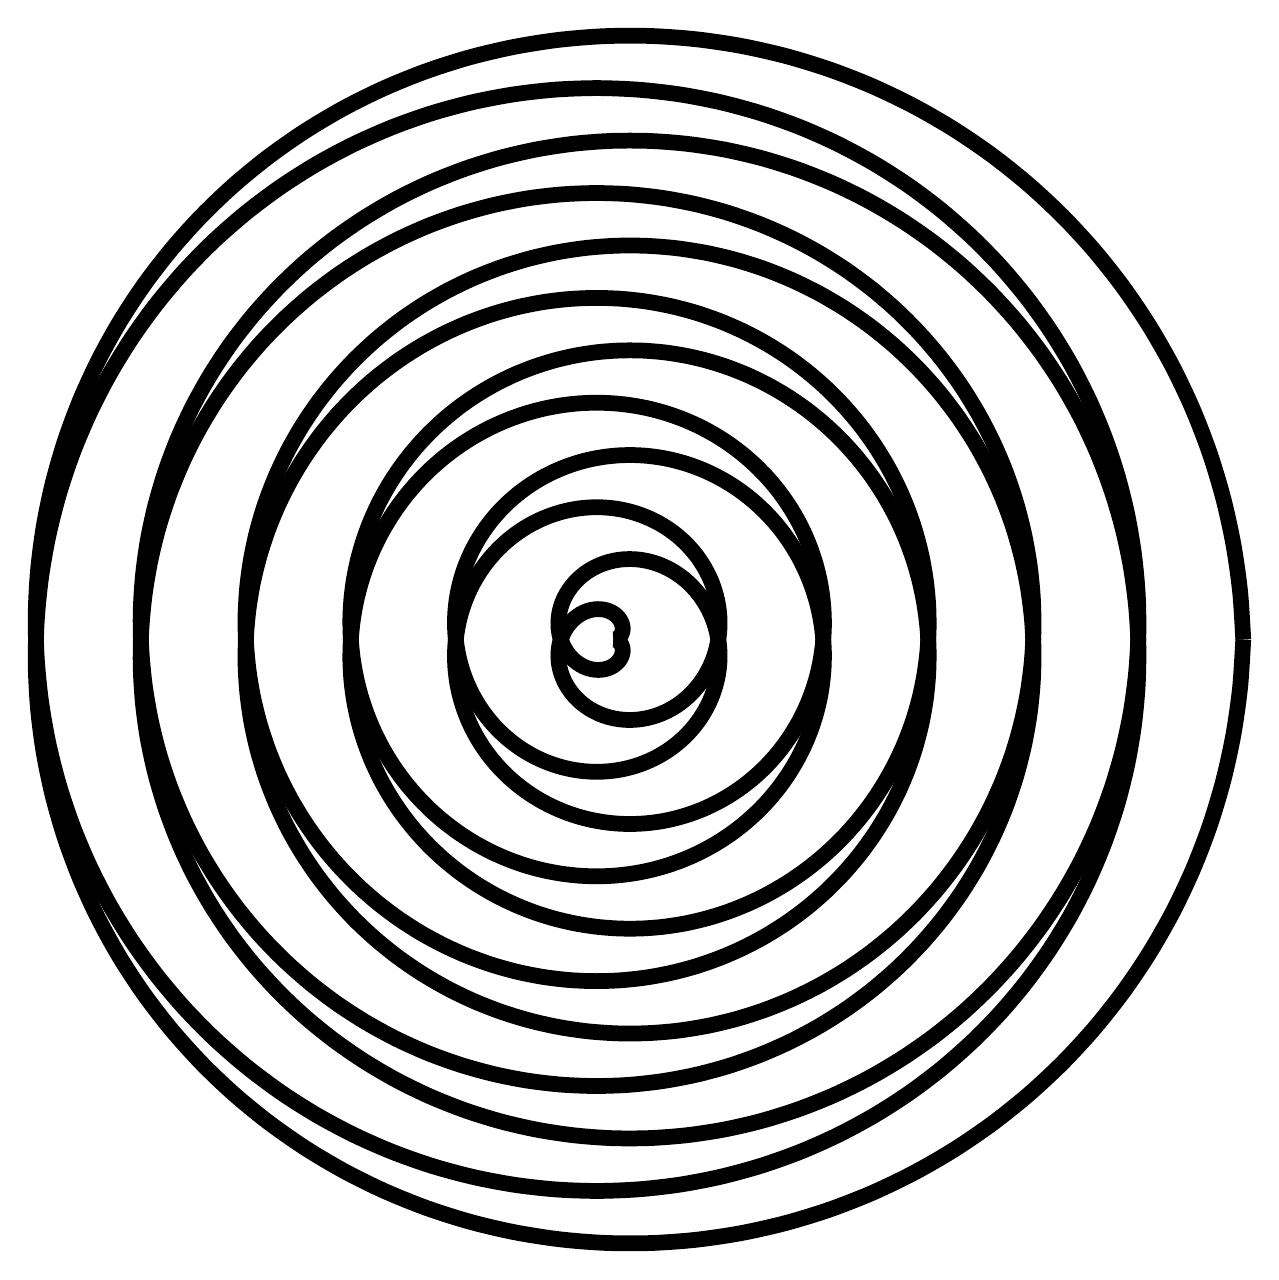
\begin{tikzpicture}
  % Defining the canvas size for the border
  \def\spiralradius{8} % Maximum radius of the spiral
  \def\spiralloops{3}  % Number of spiral loops
  \def\borderwidth{0.2cm} % Thickness of the spiral line

  % Drawing the outer spiral (clockwise)
  \draw[line width=\borderwidth, black] 
    plot[domain=0:720*\spiralloops, samples=500, smooth] 
    ({\spiralradius*(1-\x/(720*\spiralloops))*cos(\x)}, 
     {\spiralradius*(1-\x/(720*\spiralloops))*sin(\x)});

  % Drawing the inner spiral (counter-clockwise) for a double-spiral effect
  \draw[line width=\borderwidth, black] 
    plot[domain=0:720*\spiralloops, samples=500, smooth] 
    ({\spiralradius*(1-\x/(720*\spiralloops))*cos(-\x)}, 
     {\spiralradius*(1-\x/(720*\spiralloops))*sin(-\x)});
\end{tikzpicture}

\vspace{1cm}

{\Huge \textbf{Ansible for DevOps}\par}

\vspace{0.5cm}

{\Large A Practical Guide to Automation for Developers and Sysadmins\par}

\vspace{1cm}

{\Large Jeff Geerling\par}

\vspace{2cm}

{\large Published by Midwestern Mac, LLC\par}
\end{center}
\clearpage

